\documentclass[10pt]{beamer}
\usepackage{textpos}
\usepackage{graphicx}
\usepackage{soul}
\usepackage{xcolor,colortbl}
\usepackage{listings}
\usepackage{lipsum}
\usepackage{ragged2e}
%
\definecolor{codegreen}{rgb}{0,0.6,0}
\definecolor{codegray}{rgb}{0.5,0.5,0.5}
\definecolor{codepurple}{rgb}{0.58,0,0.82}
\definecolor{backcolour}{rgb}{0.95,0.95,0.92}
\definecolor{nbackcolour}{rgb}{0.75,1,1}
\definecolor{darkblue}{rgb}{0.1,0.1,0.5}
\definecolor{outputboxcolor}{rgb}{0.2,0.3,0.5}
\definecolor{lightcyan}{rgb}{0.3,0.97,0.97}
\definecolor{dgreen}{rgb}{0,0.6,0.3}
\definecolor{lblue}{rgb}{0,0.65,1}
%
\lstdefinestyle{mystyle}{
    backgroundcolor=\color{nbackcolour},   
    commentstyle=\scriptsize\color{codegreen},
    keywordstyle=\color{magenta},
    numberstyle=\tiny\color{codegray},
    stringstyle=\color{codepurple},
    basicstyle=\ttfamily\scriptsize,
    breakatwhitespace=false,         
    breaklines=true,                 
    captionpos=b,                    
    keepspaces=true,                 
    numbers=left,                    
    numbersep=5pt,                  
    showspaces=false,                
    showstringspaces=false,
    showtabs=false,                  
    tabsize=2,
    xleftmargin=10pt,
    xrightmargin=6pt,
    columns=flexible
}
\lstset{style=mystyle}
%
% Change example block colors
% 1- Block title (background and text)
\setbeamercolor{block title example}{fg=white, bg=blue}
% 2- Block body (background and text)
\setbeamercolor{block body example}{bg=teal!25}
% Change alert block colors
% 1- Block title (background and text)
\setbeamercolor{block title alerted}{fg=cyan, bg=orange}
% 2- Block body (background and text)
\setbeamercolor{block body alerted}{bg=orange!25}
% Change standard block colors
% 1- Block title (background and text)
\setbeamercolor{block title}{bg=purple, fg=white}
% 2- Block body (background)
\setbeamercolor{block body}{bg=cyan!10}
%
\usetheme{IPG}
%
\setbeamerfont{frametitle}{size=\large}
\setbeamerfont{block title}{size=\small}
\setbeamerfont{block title example}{size=\small}
\setbeamerfont{block title alerted}{size=\small}
\setbeamerfont{block body}{size=\small}
\setbeamerfont{block body example}{size=\small}
\setbeamerfont{block body alerted}{size=\small}
%
\author[miladmolaee@hotmail.com]{\large Milad Molaee}
% 
\title[C++ Programming]{C++ Programming\\\vspace{5pt}from Beginner to Expert\\\vspace{20pt}{\color{darkblue}\large Chapter 7: Functions and an Introduction to Recursion}}
%
\begin{document} 
%
\setbeamercolor{itemize item}{fg=red}
\frame{\titlepage}

%
\begin{frame}{Outline}
\footnotesize\tableofcontents
\end{frame}


\section{Introduction}
\begin{frame}{Introduction}
	\justifying
	Experience has shown that the best way to develop and maintain large programs is to construct them from small, simple pieces, or components. This technique is
	called \textbf{divide and conquer}.
	\\\vspace{10pt}
	\begin{center}
		\begin{figure}
			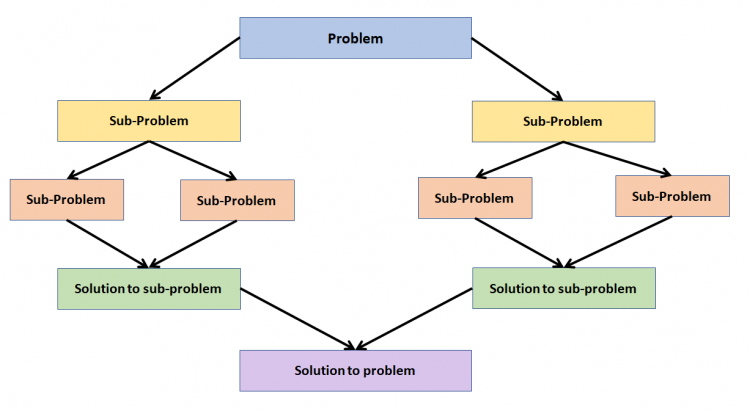
\includegraphics[width=0.7\linewidth]{./.images/.img-6-1.png}
			\caption{Divide and Conquer Algorithm}
		\end{figure}
	\end{center}
\end{frame}


\begin{frame}{Introduction}
	\justifying
	\begin{itemize}
		\setlength\itemsep{0.5em}
		\item [\color{purple}\blacksquare] A function is a block of code which \underline{only runs when it is called}.
		\item [\color{purple}\blacksquare] You can \underline{pass data}, known as parameters, into a function.
		\item [\color{purple}\blacksquare] Functions are used to perform certain actions, and they are important for \underline{reusing code}: Define the code once, and use it many times.
		\\\vspace{10pt}
		C++ provides some \textbf{pre-defined functions}, such as \texttt{\color{blue}main()}, which is used to execute code. But you can also create your own functions to perform certain actions.
		\\\vspace{8pt}
		\lstinputlisting[language=C++,firstline=1,lastline=6,numbers=none]{./.codes/.codes.cpp}
	\end{itemize}
\end{frame}


\begin{frame}
	\justifying
	\small
		Functions allow you to \textbf{modularize a program by separating its tasks} into self-contained units. You’ve used a \textbf{combination of library functions and your own functions} in	almost every program you’ve written.
	\begin{center}
		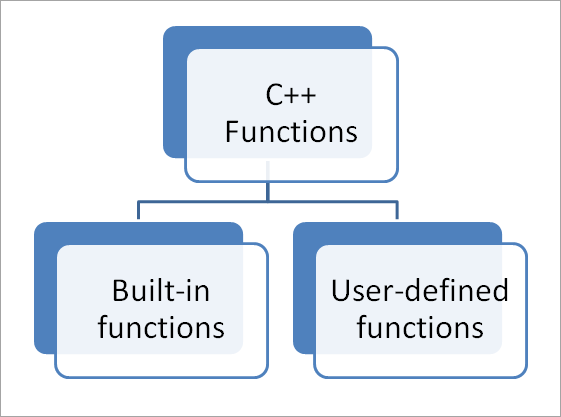
\includegraphics[width=4cm]{./.images/.img-6-2.png}
	\end{center}
\small The C++	Standard Library provides a rich collection of functions for \textbf{common mathematical calculations, string manipulations, character manipulations, input/output, error checking} and many other useful operations.
\end{frame}





\section{Program Components in C++}
\begin{frame}{Standard Template Library in C++}
	\begin{itemize}
		\small
		\item [\color{purple}\blacksquare] Container
		\begin{itemize}
			\item [$\bullet$] Sequence Container
			\item [$\bullet$] Associative Container
			\item [$\bullet$] Container Adapter
			\item [$\bullet$] Unordered Associative Container
		\end{itemize}
	\item [\color{purple}\blacksquare] Iterator
	\begin{itemize}
		\item [$\bullet$] \texttt{begin()}
		\item [$\bullet$] \texttt{next()}
		\item [$\bullet$] \texttt{prev()}
		\item [$\bullet$] \texttt{advance()}
		\item [$\bullet$] \texttt{end()}
	\end{itemize}
	\item [\color{purple}\blacksquare] Algorithm
	\begin{itemize}
		\item [$\bullet$] Sorting and Searching Algorithm
		\item [$\bullet$] minimum and maximum Operation
		\item [$\bullet$] Numeric Algorithm
		\item [$\bullet$] Modifying and non-modifying Algorithm
	\end{itemize}
	\end{itemize}
\end{frame}
	
	
\begin{frame}{\normalsize Hierarchical boss-function/worker-function relationship}
	\begin{center}
		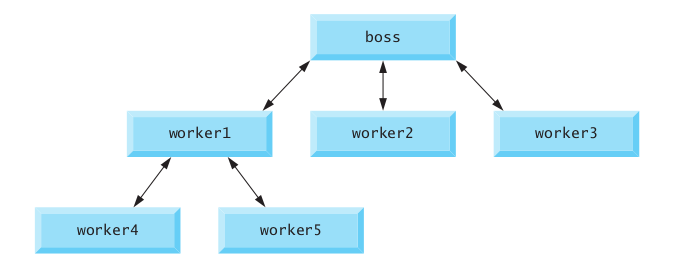
\includegraphics[width=8cm]{./.images/.img-6-3.png}
	\end{center}
\vspace{15pt}
\begin{exampleblock}{Example}
	\small\justifying
	A boss (similar to the calling function) asks a worker (similar to a called function) to
	perform a task and report back (i.e., return) the results after completing the task. The boss
	function does not know how the worker function performs its designated tasks. The
	worker may also call other worker functions, unbeknownst to the boss.
\end{exampleblock}	
\end{frame}




\section{Math Library Functions}
\begin{frame}{Math Library Functions}
	\justifying
	{\small Some functions, such as main, are not members of a class. These functions are called \textbf{global	functions}. For example The \texttt{\color{blue}<cmath>} header provides a collection of functions that perform common mathematical calculations. For example, you can calculate the square root of \texttt{900.0} with the	function call:}
\\
	\lstinputlisting[language=C++,firstline=26,lastline=26,numbers=none]{./.codes/.codes.cpp}
	\\
	{\small This expression evaluates to \texttt{30.0}. Function \texttt{sqrt} takes an argument of type \texttt{double} and returns a \texttt{double} result.\\\vspace{15pt}
	Function arguments may be \textbf{constants}, \textbf{variables} or \textbf{\underline{more complex expressions}}. \\If
	\texttt{c = 13.0}, \texttt{d = 3.0} and \texttt{f = 4.0}, then the statement:}
\\
	\lstinputlisting[language=C++,firstline=27,lastline=27,numbers=none]{./.codes/.codes.cpp}
	{\small displays the square root of \texttt{13.0 + 3.0 * 4.0 = 25.0}—namely, \texttt{5.0}.}
\end{frame}

\begin{frame}
	\centering\scriptsize\renewcommand{\arraystretch}{1.5}
	\begin{tabular}{p{0.1\linewidth} p{0.5\linewidth} p{0.25\linewidth}}
		\hline
		\rowcolor{cyan}\color{white} Function & \color{white} Description & \color{white} Example \\\hline
		
		\rowcolor{lightcyan} \texttt{ceil(x)} & rounds $x$ to the smallest integer not less than $x$ & 
		\texttt{ceil(9.2)} is \texttt{10.0}
		
		\texttt{ceil(-9.8)} is \texttt{-9.0}\\\hline
		
		
		\rowcolor{lightcyan} \texttt{cos(x)} & trigonometric cosine of $x$ ($x$ in radians) & \texttt{cos(0.0)} is \texttt{1.0} \\\hline
		
		
		\rowcolor{lightcyan} \texttt{exp(x)} & exponential function $e^x$ & 
		\texttt{exp(1.0)} is \texttt{2.718282}
			
		\texttt{exp(2.0)} is \texttt{7.389056}\\\hline
		
		
		\rowcolor{lightcyan} \texttt{fabs(x)} & absolute value of $x$ & 
		\texttt{fabs(5.2)} is \texttt{5.2} 
			
		\texttt{fabs(0.0)} is \texttt{0.0} 
			
		\texttt{fabs(-1.2)} is \texttt{1.2}\\\hline
		
		
		\rowcolor{lightcyan} \texttt{floor(x)} & rounds $x$ to the largest integer not greater than $x$ & \texttt{floor(9.2)} is \texttt{9.0}
		
		
		\texttt{floor(-9.8)} is \texttt{-10.0} \\\hline
		
		
		\rowcolor{lightcyan} \texttt{fmod(x)} & remainder of $x/y$ as a floating-point number & \texttt{fmod(2.6, 1.2)} is \texttt{0.2} \\\hline
		
		
		\rowcolor{lightcyan} \texttt{log(x)} & natural logarithm of $x$ (base $e$) & 
		\texttt{log(2.718282)} is \texttt{1.0}
		
		
		\texttt{log(7.389056)} is \texttt{2.0} \\\hline
		
		
		\rowcolor{lightcyan} \texttt{log10(x)} & logarithm of $x$ (base 10) & 
		\texttt{log(10.0)} is \texttt{1.0}
		
		
		\texttt{log(100.0)} is \texttt{2.0} \\\hline
		
		
		\rowcolor{lightcyan} \texttt{pow(x)} & $x$ raised to power y ($x^y$) & 
		\texttt{pow(2, 7)} is \texttt{128}
		
		\texttt{pow(25, 0.5)} is \texttt{5} \\\hline
		
		
		\rowcolor{lightcyan} \texttt{sin(x)} & trigonometric sine of $x$ ($x$ in radians) & \texttt{sin(0.0)} is \texttt{0.0} \\\hline
		
		
		\rowcolor{lightcyan} \texttt{sqrt(x)} & square root of $x$ (where $x$ is a nonnegative value) & \texttt{sqrt(64)} is \texttt{8} \\\hline
		
		
		\rowcolor{lightcyan} \texttt{tan(x)} & trigonometric tangent of $x$	($x$ in radians) & \texttt{tan(0.0)} is \texttt{0.0} \\\hline

	\end{tabular}
\end{frame}


\section{Function Prototypes}
\begin{frame}{Function-Prototype and Argument-Coercion Notes}
	\justifying
	For a function that’s not defined in a class, you must either define the function before
	using it or you must declare that the function exists.
	\lstinputlisting[language=C++,firstline=5,lastline=5,numbers=none]{../codes/chapter-6/example-6-1/example-6-1.cpp}
\end{frame}


\begin{frame}
	\lstinputlisting[language=C++]{../codes/chapter-6/example-6-1/example-6-1.cpp}
\end{frame}


\begin{frame}
	\begin{block}{\color{white}Output}
		\texttt{Enter three integer grades: 86 67 75\\
			The maximum integer value is: 86}
	\end{block}
	\begin{block}{\color{white}Output}
		\texttt{Enter three integer grades: 67 86 75\\
			The maximum integer value is: 86}
	\end{block}
	\begin{block}{\color{white}Output}
		\texttt{Enter three integer grades: 67 75 86\\
			The maximum integer value is: 86}
	\end{block}
\end{frame}


\begin{frame}
	\justifying\small
	When compiling the program, the compiler uses the prototype to:
	\vspace{10pt}
	\begin{itemize}
		\setlength\itemsep{1em}\justifying\small
		\item Ensure that maximum’s first line (\textbf{function header}) {\footnotesize (line 17)} matches its \textbf{prototype} {\footnotesize (line 5)}.
		\item Check that the call to maximum (\textbf{function call}) {\footnotesize (line 14)} contains the correct number and types
		of arguments, and that the types of the arguments are in the correct order (in this
		case, all the arguments are of the same type).
		
		\item Ensure that the value returned by the function can be used correctly in the expression that called the function, for example, for a function that returns void
		you cannot call the function on right side of an assignment.
		
		\item Ensure that each argument is consistent with the type of the corresponding parameter, for example, a parameter of type double can receive values like 7.35, 22 or
		–0.03456, but not a string like "hello". If the arguments passed to a function do
		not match the types specified in the function’s prototype, the compiler attempts
		to convert the arguments to those types. 
	\end{itemize}
\end{frame}

\begin{frame}
	\centering\scriptsize\renewcommand{\arraystretch}{1.8}
	\begin{tabular}{p{0.238\linewidth} p{0.36\linewidth} p{0.1\linewidth}}
		
		\rowcolor{cyan}\color{white} Data types & & \color{white} Size (byte)\\
		
		\rowcolor{lightcyan} \texttt{long double} & \texttt{} & \hspace{13pt}\texttt{12}\\
		\rowcolor{lightcyan} \texttt{double} & \texttt{} & \hspace{16pt}\texttt{8}\\
		\rowcolor{lightcyan} \texttt{float} & \texttt{} & \hspace{16pt}\texttt{4}\\
		\rowcolor{lightcyan} \texttt{unsigned long long int} & synonymous with \texttt{unsigned long long} & \hspace{16pt}\texttt{8}\\
		\rowcolor{lightcyan} \texttt{long long int} & synonymous with \texttt{long long} & \hspace{16pt}\texttt{8}\\
		\rowcolor{lightcyan} \texttt{unsigned long int} & synonymous with \texttt{unsigned long} & \hspace{16pt}\texttt{4}\\
		\rowcolor{lightcyan} \texttt{long int} & synonymous with \texttt{long} & \hspace{16pt}\texttt{4}\\
		\rowcolor{lightcyan} \texttt{unsigned int} & synonymous with \texttt{unsigned} & \hspace{16pt}\texttt{4}\\
		\rowcolor{lightcyan} \texttt{int} & \texttt{} & \hspace{16pt}\texttt{4}\\
		\rowcolor{lightcyan} \texttt{unsigned short int} & synonymous with \texttt{unsigned short} & \hspace{16pt}\texttt{2}\\
		\rowcolor{lightcyan} \texttt{short int} & synonymous with \texttt{short} & \hspace{16pt}\texttt{2}\\
		\rowcolor{lightcyan} \texttt{unsigned char} & \texttt{} & \hspace{16pt}\texttt{1}\\
		\rowcolor{lightcyan} \texttt{char} & \texttt{} & \hspace{16pt}\texttt{1}\\
		\rowcolor{lightcyan} \texttt{bool} & \texttt{} & \hspace{16pt}\texttt{1}\\
		
	\end{tabular}
\end{frame}

\begin{frame}
	\centering\scriptsize\renewcommand{\arraystretch}{1.8}
	\begin{tabular}{p{0.238\linewidth} p{0.38\linewidth} p{0.1\linewidth}}
		
		\rowcolor{cyan}\color{white} Data Type & \color{white}\centering Range & \color{white} Size (byte)\\
		
		\rowcolor{lightcyan} \texttt{long double} & \centering$-1.18973\times10^{4932}$ to $1.18973\times10^{4932}$ & \hspace{13pt}\texttt{12}\\
		\rowcolor{lightcyan} \texttt{double} & \centering$-1.79769\times10^{308}$ to $1.79769\times10^{308}$ & \hspace{16pt}\texttt{8}\\
		\rowcolor{lightcyan} \texttt{float} & \centering$-3.40282e\times10^{38}$ to $3.40282\times10^{38}$ & \hspace{16pt}\texttt{4}\\
		\rowcolor{lightcyan} \texttt{unsigned long long int} & \centering$0$ to $2^{64}-1$ & \hspace{16pt}\texttt{8}\\
		\rowcolor{lightcyan} \texttt{long long int} & \centering$-(2^{63})$ to $2^{63}-1$ & \hspace{16pt}\texttt{8}\\
		\rowcolor{lightcyan} \texttt{unsigned long int} & \centering$0$ to $4,294,967,295$ & \hspace{16pt}\texttt{4}\\
		\rowcolor{lightcyan} \texttt{long int} & \centering$-2,147,483,648$ to $2,147,483,647$ & \hspace{16pt}\texttt{4}\\
		\rowcolor{lightcyan} \texttt{unsigned int} & \centering$0$ to $4,294,967,295$ & \hspace{16pt}\texttt{4}\\
		\rowcolor{lightcyan} \texttt{int} & \centering$-2,147,483,648$ to $2,147,483,647$ & \hspace{16pt}\texttt{4}\\
		\rowcolor{lightcyan} \texttt{unsigned short int} & \centering$0$ to $65,535$ & \hspace{16pt}\texttt{2}\\
		\rowcolor{lightcyan} \texttt{short int} & \centering$-32,768$ to $32,767$ & \hspace{16pt}\texttt{2}\\
		\rowcolor{lightcyan} \texttt{unsigned char} & \centering$0$ to $255$ & \hspace{16pt}\texttt{1}\\
		\rowcolor{lightcyan} \texttt{char} & \centering$-128$ to $127$ & \hspace{16pt}\texttt{1}\\
		\rowcolor{lightcyan} \texttt{bool} & \centering\texttt{true / false} & \hspace{16pt}\texttt{1}\\
	\end{tabular}
\end{frame}

\section{C++ Standard Library Headers}
\begin{frame}{C++ Standard Library Headers}
	\lipsum[2]
\end{frame}

\begin{frame}
	{Standard Template Library - Part 1\vspace{5pt}}
	\centering\scriptsize\renewcommand{\arraystretch}{2}
	\begin{tabular}{p{0.22\linewidth} p{0.7\linewidth}}
		
		\rowcolor{cyan}\color{white} Standard Library header & \color{white} Explanation\\
		
		\rowcolor{lightcyan} \texttt{<iostream>} & Contains function prototypes for the C++ standard input and output functions. \\
		\rowcolor{lightcyan} \texttt{<iomanip>} & Contains function prototypes for stream manipulators that format streams of data. \\
		\rowcolor{lightcyan} \texttt{<cmath>} & Contains function prototypes for math library functions. \\
		\rowcolor{lightcyan} \texttt{<cstdlib>} & Contains function prototypes for conversions of numbers to text, text to numbers, memory allocation, random numbers and various other utility functions. \\
		\rowcolor{lightcyan} \texttt{<ctime>} & Contains function prototypes and types for manipulating the time and date. \\
		\rowcolor{lightcyan} \texttt{<array>,
			<vector>, <list>,
			<forward\_list>,
			<deque>, <queue>,
			<stack>, <map>,
			<unordered\_map>,
			<unordered\_set>,
			<set>, <bit\_set>} & These headers contain classes that implement the C++ Standard Library
		containers. Containers store data during a program’s execution. 
		
		A container is a holder object that stores a collection of other objects (its elements). They are implemented as class templates, which allows great flexibility in the types supported as elements. 
		
		The container manages the storage space for its elements and provides member functions to access them, either directly or through iterators (reference objects with similar properties to pointers). 
	\end{tabular}
\end{frame}

\begin{frame}
	{Standard Template Library - Part 2}
	\centering\scriptsize\renewcommand{\arraystretch}{2}
	\begin{tabular}{p{0.22\linewidth} p{0.7\linewidth}}
		
		\rowcolor{cyan}\color{white} Standard Library header & \color{white} Explanation\\
		
		\rowcolor{lightcyan} \texttt{<cctype>} & Contains function prototypes for functions that test characters for certain properties (such as whether the character is a digit or a punctuation), and function prototypes for functions that can be used to convert
		lowercase letters to uppercase letters and vice versa. \\
		\rowcolor{lightcyan} \texttt{<cstring>} & Contains function prototypes for C-style string-processing functions. \\
		\rowcolor{lightcyan} \texttt{<typeinfo>} & Contains classes for runtime type identification (determining data types	at execution time). \\
		\rowcolor{lightcyan} \texttt{<exception>, <stdexcept>} & These headers contain classes that are used for exception handling. \\
		\rowcolor{lightcyan} \texttt{<memory>} & Contains classes and functions used by the C++ Standard Library to allocate memory to the C++ Standard Library containers. \\
		\rowcolor{lightcyan} \texttt{<fstream>} & Contains function prototypes for functions that perform input from and output to files on disk. \\
		\rowcolor{lightcyan} \texttt{<string>} & Contains the definition of class string from the C++ Standard Library. \\
		\rowcolor{lightcyan} \texttt{<sstream>} & Contains function prototypes for functions that perform input from strings in memory and output to strings in memory.	
	\end{tabular}
\end{frame}

\begin{frame}{Standard Template Library - Part 3}
	\centering\scriptsize\renewcommand{\arraystretch}{1.8}
	\begin{tabular}{p{0.22\linewidth} p{0.7\linewidth}}
		
		\rowcolor{cyan}\color{white} Standard Library header & \color{white} Explanation\\
		
		\rowcolor{lightcyan} \texttt{<functional>} & Contains classes and functions used by C++ Standard Library algorithms. \\	
		\rowcolor{lightcyan} \texttt{<iterator>} & Contains classes for accessing data in the C++ Standard Library containers. \\
		\rowcolor{lightcyan} \texttt{<algorithm>} & Contains functions for manipulating data in C++ Standard Library containers. \\
		\rowcolor{lightcyan} \texttt{<cassert>} & Contains macros for adding diagnostics that aid program debugging. \\
		\rowcolor{lightcyan} \texttt{<cfloat>} & Contains the floating-point size limits of the system. \\
		\rowcolor{lightcyan} \texttt{<climits>} & Contains the integral size limits of the system. \\
		\rowcolor{lightcyan} \texttt{<cstdio>} & Contains function prototypes for the C-style standard input/output library functions. \\
		\rowcolor{lightcyan} \texttt{<local>} & Contains classes and functions normally used by stream processing to		process data in the natural form for different languages (e.g., monetary		formats, sorting strings, character presentation, etc.). \\
		\rowcolor{lightcyan} \texttt{<limits>} & Contains classes for defining the numerical data type limits on each	computer platform—this is C++’s version of <climits> and <cfloat>. \\
		\rowcolor{lightcyan} \texttt{<utility>} & Contains classes and functions that are used by many C++ Standard		Library headers.
	\end{tabular}
\end{frame}


\section{Random-Number Generation}
\begin{frame}{Random-Number Generation}
	The element of chance can be introduced into computer applications by using the
	C++ Standard Library function rand. Consider the following statement:
	
	\lstinputlisting[language=C++,firstline=29,lastline=29,numbers=none]{./.codes/.codes.cpp}
	
	The function rand generates an unsigned integer between 0 and \texttt{RAND\_MAX} (a symbolic
	constant defined in the \texttt{<cstdlib>} header). You can determine the value of \texttt{RAND\_MAX} for
	your system simply by displaying the constant. If rand truly produces integers at random,
	every number between 0 and \texttt{RAND\_MAX} has an equal chance (or probability) of being chosen each time rand is called.\\\vspace{10pt}
	
	To produce integers in the range 0 to 5, we use the remainder operator (\%) with rand as follows:
	
	\lstinputlisting[language=C++,firstline=31,lastline=31,numbers=none]{./.codes/.codes.cpp}
	
	This is called scaling. The number 6 is called the scaling factor.
\end{frame}

\begin{frame}
	\lstinputlisting[language=C++]{../codes/chapter-6/example-6-2/example-6-2.cpp}
\end{frame}

\begin{frame}
	\lstinputlisting[language=C++,lastline=29]{../codes/chapter-6/example-6-3/example-6-3.cpp}
\end{frame}

\begin{frame}
	\lstinputlisting[language=C++,firstline=30,firstnumber=30]{../codes/chapter-6/example-6-3/example-6-3.cpp}
\end{frame}

\begin{frame}
	\lstinputlisting[language=C++]{../codes/chapter-6/example-6-4/example-6-4.cpp}
\end{frame}

\begin{frame}{\small Seeding the Random-Number Generator with the Current Time}
	To randomize without having to enter a seed each time, we can use a statement like
	
	\lstinputlisting[firstline=33,lastline=33,numbers=none]{./.codes/.codes.cpp}
	
	This causes the computer to read its clock to obtain the value for the seed. Function time
	(with the argument 0 as written in the preceding statement) typically returns the current
	time as the number of seconds since January 1, 1970, at midnight Greenwich Mean Time
	(GMT). This value (which is of type time\_t) is converted to an unsigned int and used as
	the seed to the random-number generator—the static\_cast in the preceding statement
	eliminates a compiler warning that’s issued if you pass a time\_t value to a function that
	expects an unsigned int. The function prototype for time is in <ctime>.
\end{frame}

\begin{frame}
	Previously, we simulated the rolling of a six-sided die with the statement
	
	\lstinputlisting[language=C++,firstline=35,lastline=35,numbers=none]{./.codes/.codes.cpp}
	
	which always assigns an integer (at random) to variable face in the range 1 ≤ face ≤ 6.
	The width of this range (i.e., the number of consecutive integers in the range) is 6 and the
	starting number in the range is 1. Referring to the preceding statement, we see that the
	width of the range is determined by the number used to scale rand with the remainder operator (i.e., 6), and the starting number of the range is equal to the number (i.e., 1) that is
	added to the expression rand \% 6. We can generalize this result as
	
	\lstinputlisting[language=C++,firstline=37,lastline=37,numbers=none]{./.codes/.codes.cpp}
	
	where the shiftingValue is equal to the first number in the desired range of consecutive integers and the scalingFactor is equal to the width of the desired range of consecutive integers.
\end{frame}

\begin{frame}{\small Case Study: Game of Chance; Introducing Scoped	enums}
	
	\begin{block}{\color{white}Question}
		A player rolls two dice. Each die has six faces. These faces contain 1, 2, 3, 4, 5 and 6
		spots. After the dice have come to rest, the sum of the spots on the two upward faces is
		calculated. If the sum is 7 or 11 on the first roll, the player wins. If the sum is 2, 3 or
		12 on the first roll (called “craps”), the player loses (i.e., the “house” wins). If the sum
		is 4, 5, 6, 8, 9 or 10 on the first roll, then that sum becomes the player’s “point.” To
		win, you must continue rolling the dice until you “make your point.” The player loses
		by rolling a 7 before making the point.
	\end{block}
\end{frame}

\begin{frame}
	
	{\scriptsize \textbf{Answer - Part 1}}
	\lstinputlisting[language=C++,lastline=30]{../codes/chapter-6/example-6-5/example-6-5.cpp}
\end{frame}
\begin{frame}
	
	{\scriptsize \textbf{Answer - Part 2}}
	\lstinputlisting[language=C++,firstline=31,lastline=60,firstnumber=31]{../codes/chapter-6/example-6-5/example-6-5.cpp}
\end{frame}
\begin{frame}
	
	{\scriptsize \textbf{Answer - Part 3}}
	\lstinputlisting[language=C++,firstline=61,firstnumber=61]{../codes/chapter-6/example-6-5/example-6-5.cpp}
\end{frame}

\begin{frame}
	\begin{block}{\color{white}Output of run 1}
		\texttt{Player rolled 2 + 5 = 7\\
			Player wins}
	\end{block}
	\begin{block}{\color{white}Output of run 2}
		\texttt{Player rolled 3 + 3 = 6\\
			Point is 6\\
			Player rolled 5 + 3 = 8\\
			Player rolled 4 + 5 = 9\\
			Player rolled 2 + 1 = 3\\
			Player rolled 1 + 5 = 6\\
			Player wins}
	\end{block}
\end{frame}

\begin{frame}
	\begin{block}{\color{white}Output of run 3}
		\texttt{Player rolled 6 + 6 = 12\\
			Player loses}
	\end{block}
	\begin{block}{\color{white}Output of run 4}
		\texttt{Player rolled 1 + 3 = 4\\
			Point is 4\\
			Player rolled 4 + 6 = 10\\
			Player rolled 2 + 4 = 6\\
			Player rolled 6 + 4 = 10\\
			Player rolled 2 + 3 = 5\\
			Player rolled 2 + 4 = 6\\
			Player rolled 1 + 1 = 2\\
			Player rolled 4 + 4 = 8\\
			Player rolled 4 + 3 = 7\\
			Player loses}
	\end{block}
\end{frame}


\section{C++11 Random Numbers}
\begin{frame}{C++11 Random Numbers}
	\lstinputlisting[language=C++]{../codes/chapter-6/example-6-6/example-6-6.cpp}
\end{frame}

\section{Scope Rules}
\begin{frame}{Scope Rules}
	\lipsum[2]
\end{frame}

\section{Function-Call Stack and Activation Records}
\begin{frame}{Function-Call Stack and Activation Records}
	\lipsum[2]
\end{frame}

\section{Inline Functions}
\begin{frame}{Inline Functions}
	Implementing a program as a set of functions is good from a software engineering stand-point, but function calls involve execution-time overhead. C++ provides inline functions to
	help reduce function-call overhead. Placing the qualifier inline before a function’s return
	type in the function definition advises the compiler to generate a copy of the function’s body
	code in every place where the function is called (when appropriate) to avoid a function call.
	This often makes the program larger. The compiler can ignore the inline qualifier and generally does so for all but the smallest functions. Reusable inline functions are typically placed
	in headers, so that their definitions can be included in each source file that uses them.
\end{frame}

\section{References and Reference Parameters}
\begin{frame}{References and Reference Parameters}
	\lipsum[2]
\end{frame}

\section{Default Arguments}
\begin{frame}{Default Arguments}
	\lipsum[2]
\end{frame}

\section{Unary Scope Resolution Operator}
\begin{frame}{Unary Scope Resolution Operator}
	\lipsum[2]
\end{frame}

\section{Function Overloading}
\begin{frame}{Function Overloading}
	\lipsum[2]
\end{frame}

\section{Function Templates}
\begin{frame}{Function Templates}
	\lipsum[2]
\end{frame}

\section{Recursion}
\begin{frame}{Recursion}
	\lipsum[2]
\end{frame}

\section{Example Using Recursion: Fibonacci Series}
\begin{frame}{Example Using Recursion: Fibonacci Series}
	\lipsum[2]
\end{frame}

\section{Recursion vs. Iteration}
\begin{frame}{Recursion vs. Iteration}
	\lipsum[2]
\end{frame}

\section{Summery and Conclusion}

\begin{frame}{Summery and Conclusion}
	\lipsum[2]
\end{frame}


\section{Exercises}

\begin{frame}{Exercises}
	\lipsum[2]
\end{frame}

\begin{frame}{\small First Program in C++: Printing a Line of Text}
	
	Consider a simple program that prints a line of text (Fig. 2.1). This program illustrates several important features of the C++ language. The text in lines 1–10 is the program’s source code. The line numbers are not part of the source code.
	
	\lstinputlisting[language=C++]{../codes/chapter-2/fig_2-1/fig_2-1.cpp}
	
	\begin{block}{\textcolor{white}{output}}
		\texttt{\small Welcome to C++!}
	\end{block}
	
\end{frame}


\begin{frame}{\small The Stream Insertion Operator and Escape Sequences}
	\centering\tiny\renewcommand{\arraystretch}{2}	
\begin{tabular}{p{0.15\linewidth} p{0.6\linewidth}}
	\rowcolor{cyan}\color{white} Escape sequence & \color{white} Description \\
	
	\rowcolor{lightcyan} $\backslash$n & Newline. Position the screen cursor to the beginning of the next line.\\ 
	
	\rowcolor{lightcyan} $\backslash$t & Horizontal tab. Move the screen cursor to the next tab stop.\\ 
	
	\rowcolor{lightcyan} $\backslash$r & Carriage return. Position the screen cursor to the beginning of the current line; do not advance to the next line.\\ 
	
	\rowcolor{lightcyan} $\backslash$a & Alert. Sound the system bell.\\ 
	
	\rowcolor{lightcyan} $\backslash\backslash$ & Backslash. Used to print a backslash character.\\ 
	
	\rowcolor{lightcyan} $\backslash$' & Single quote. Used to print a single-quote character.\\ 
	
	\rowcolor{lightcyan} $\backslash$" & Double quote. Used to print a double-quote character.
\end{tabular}
\end{frame}


\begin{frame}{\small Arithmetic Operators}
	\centering\tiny\renewcommand{\arraystretch}{2}
	\begin{tabular}{p{0.15\linewidth} p{0.16\linewidth} p{0.2\linewidth} p{0.2\linewidth}}
		
		\rowcolor{cyan}\color{white} Operation & \color{white} Arithmetic operator & \color{white} Algebraic expression & \color{white} C++ expression \\
		
		\rowcolor{lightcyan} Addition & + & $f + 7$ & \texttt{f + 7} \\
		
		\rowcolor{lightcyan} Subtraction & - & $p - c$ & \texttt{p - c} \\
		
		\rowcolor{lightcyan} Multiplication & * & $bm$ or $b \cdot m$ & \texttt{b * m} \\
		
		\rowcolor{lightcyan} Division & / & $\dfrac{x}{y}$ or $x/y$ or $x\div y$ & \texttt{x / y} \\
		
		\rowcolor{lightcyan} Remainder & \% & $r$ $mod$ $s$ & \texttt{r \% s} 
	\end{tabular}
\end{frame}


\begin{frame}{\small Precedence of Arithmetic Operators}
	\centering\tiny\renewcommand{\arraystretch}{2}
	\begin{tabular}{p{0.12\linewidth} p{0.13\linewidth} p{0.65\linewidth}}
		
		\rowcolor{cyan}\color{white} Operator(s) & \color{white} Operation(s) & \color{white} Order of evaluation (precedence) \\\hline
		
		\rowcolor{lightcyan} \texttt{( )} & Parentheses & Evaluated first. For nested parentheses, such as in the expression
		\texttt{a * (b + c / (d + e))}, the expression in the innermost pair evalu ates first.\newline[Caution: If you have an expression such as \texttt{(a + b) * (c - d)} in which two sets of parentheses are not nested, but appear “on the same level,” the C++ Standard does not specify the order in which these parenthesized subexpressions will evaluate.] \\\hline
		
		\rowcolor{lightcyan} \texttt{*}\newline\texttt{/} \newline \texttt{\%} & Multiplication \newline Division \newline Remainder & Evaluated second. If there are several, they’re evaluated left to right. \\\hline
		
		\rowcolor{lightcyan} \texttt{+}\newline\texttt{-} & Addition \newline Subtraction & Evaluated last. If there are several, they’re evaluated left to right. \\\hline	
	\end{tabular}
\end{frame}



\begin{frame}{\small Decision Making: Equality and Relational Operators}
	\centering\tiny\renewcommand{\arraystretch}{2}
	\begin{tabular}{p{0.15\linewidth} p{0.15\linewidth} p{0.2\linewidth} p{0.25\linewidth}}
		
		\rowcolor{cyan}\color{white} Algebraic relational or equality operator & \color{white} C++ relational or equality operator & \color{white} Sample C++ condition & \color{white} Meaning of C++ condition \\\hline
		
		\rowcolor{lightcyan} \multicolumn{4}{l}{Relational operators} \\
		
		\rowcolor{lightcyan} $>$ & \texttt{>} & \texttt{x > y} & x is greater than y \\
		
		\rowcolor{lightcyan} $<$ & \texttt{<} & \texttt{x < y} & x is less than y \\
		
		\rowcolor{lightcyan} $\geq$ & \texttt{>=} & \texttt{x >= y} or & x is greater than or equal to y \\
		
		\rowcolor{lightcyan} $\leq$ & \texttt{<=} & \texttt{x <= y} & x is less than or equal to y \\\hline
		
		\rowcolor{lightcyan} \multicolumn{4}{l}{Equality operators} \\
		
		\rowcolor{lightcyan} $=$ & \texttt{==} & \texttt{x == y} & x is equal to y \\
		
		\rowcolor{lightcyan} $\neq$ & \texttt{!=} & \texttt{x != y} & x is not equal to y \\\hline
	\end{tabular}
\end{frame}


%
\end{document} 